\documentclass{article}

\usepackage{fancyhdr}
\usepackage{ragged2e}
\usepackage{graphicx}
\usepackage{caption}
\usepackage{geometry}
\usepackage{amsmath}
\usepackage{rotating}

\usepackage{listings}
\usepackage{color}

\definecolor{dkgreen}{rgb}{0,0.6,0}
\definecolor{gray}{rgb}{0.5,0.5,0.5}
\definecolor{mauve}{rgb}{0.58,0,0.82}

\lstset{frame=tb,
  language=Java,
  aboveskip=3mm,
  belowskip=3mm,
  showstringspaces=false,
  columns=flexible,
  basicstyle={\small\ttfamily},
  numbers=none,
  numberstyle=\tiny\color{gray},
  keywordstyle=\color{blue},
  commentstyle=\color{dkgreen},
  stringstyle=\color{mauve},
  breaklines=true,
  breakatwhitespace=true,
  tabsize=4
}

\setcounter{secnumdepth}{1}

\usepackage{chngcntr}
\counterwithin{figure}{section}

\renewcommand*{\thepage}{C\arabic{page}}

\pagestyle{fancy}
\lhead{ACME Robotics}
\chead{\#8367}
\rhead{\ifcontents Contents \else Week \thesection \fi}

\newif\ifcontents
\contentstrue

\makeatletter
\renewcommand{\@seccntformat}[1]{}
\makeatother

\begin{document}\contentsfalse

\begin{figure}
    \centering
    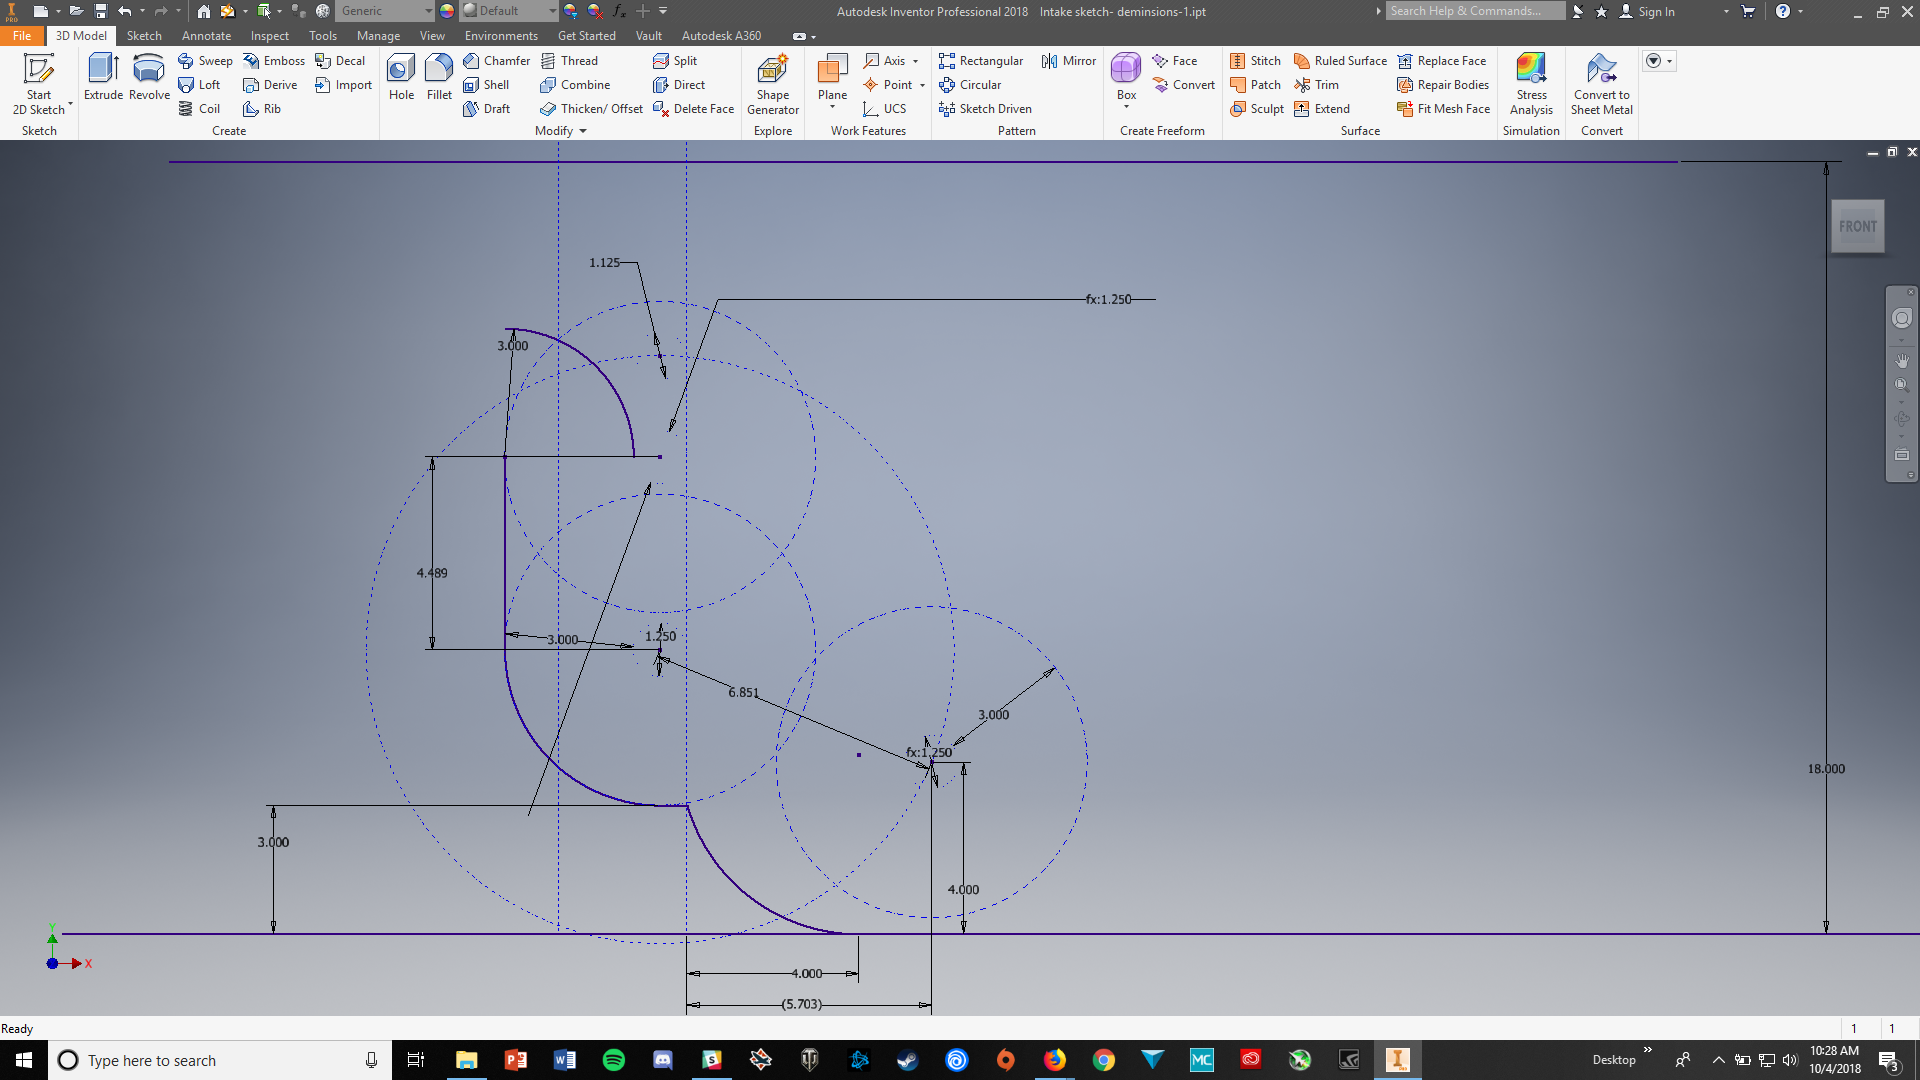
\includegraphics[width=.6\textwidth]{02_09-10/images/intakesketch.png}
    \caption{Deploy-able intake dimensions}
    \label{fig:intake}
\end{figure}

\subsection{Develop intake prototypes}
%!The game this year requires the robot to be able to sort the gold and silver minerals. We need to come up with and test various ideas for ways to pick up and sort out the two types of minerals.
After the whole team watched the game video, several members began prototyping mechanisms to intake and sort cubes. Because the game requires the robot to pick up minerals that are inside the crater, the robot either needs to be able to climb over the crater to intake the minerals, or extend some sort of intake over the crater wall. 

we decided to try developing an intake mechanism that would allow the robot to stay outside of the crater, and reach over the wall, which would allow the team to continue using a mecanum drivetrain, for its increased maneuverability. The first concept they thought of was to extend a rake in front of the robot, on linear slides, that would pull the minerals back to the robot and up the crater wall. The rake would have tines spaced a little bit under 2.75 in apart, so the silver minerals would be pulled back, but not the gold minerals. This would allow the robot to cycle back and fourth between the crater and the silver depot, to score minerals as fast as possible. When this prototype was tested, Kelly found that the gold minerals could still be pulled back, when a silver mineral would get stuck in the tines of the rake, so the rake concept would not work to sort out the minerals. 

The next concept Kelly tested was a spinning surgical-tubing intake, similar to ACME's Velocity Vortex robot. By spinning the two stages of the intake in opposite directions, the minerals would first be pulled into the robot, and then pushed against the rake, expelling the gold minerals and allowing the silver to pass into the robot. This design relied on the fact that if the intake was extended over the outer boarder of the crater, any minerals in it would be inside the crater, and thus not subject to the two mineral maximum. This worked well to pull in the minerals once they were brought to the top of the crater wall by the rake, but the transition between the two counter-rotating brushes caused the minerals to get stuck, or rejected prematurely. 

After watching videos of robots from Res-Q, the last FTC game to involve the same game elements, Kelly decided the surgical tubing intake was worth pursuing, because it could quickly bring minerals to the top of the robot one at a time, which would be necessary for sorting them out. Kelly built a new prototype that had the surgical tubing whips mounted directly over one another and rotating the same direction. Ashlin built a acrylic back plate and funnel that would guide the minerals up the intake, and allow only one to pass through the top at once. Kelly built a simple sorting system that consisted of two parallel bars mounted far enough apart to allow the gold to pass through, but not the silver. When this was combined with the spinning intake, the minerals would be sucked up into the robot, and then divided into gold and silver. 

After Jon finished the prototype for the intake he began to find the optimum distances the needed to be from the ground, crater edge, and edge of the robot. This is because these measurements are vital for CADing and fabrication. Jon found that the optimum distance from the robot to the roller was 7 inches. While the optimum distance from the floor to the roller was 4 inches. 




\subsection{Investigate possible drivetrain designs}
%! Research different drivetrains and decide which would be suitable for this game.
Given that a good drivetrain is vital for a successful robot, the team needed a solid design. The team decided there were two ways of going about creating a good drivetrain for the Rover Ruckus challenge. The first was to design a drivetrain capable of going inside the crater. The team thought this might be a good idea seeing as the intake design would be simpler and we could traverse all areas of play. This would need to be a drivetrain with very good traction, torque, and durability. For this purpose the team looked into a drop-center tank design (WCD) or a tracked design. Suspension was also considered. These were considered because both WCD and tracked designs are very effective at traversing rough or bumpy terrain. Like the crater rim. Jon did research in this area and found a simple suspension (bell crank) design and sketched a few ideas for a tracked drive train (fig 0.1). After discussing these together, and WCD, the team decided that going into the crater was probably not necessary. Thus, the team stopped development on these ideas and continued pursing the second way of going about designing a drive train.



\begin{figure}
    \centering
    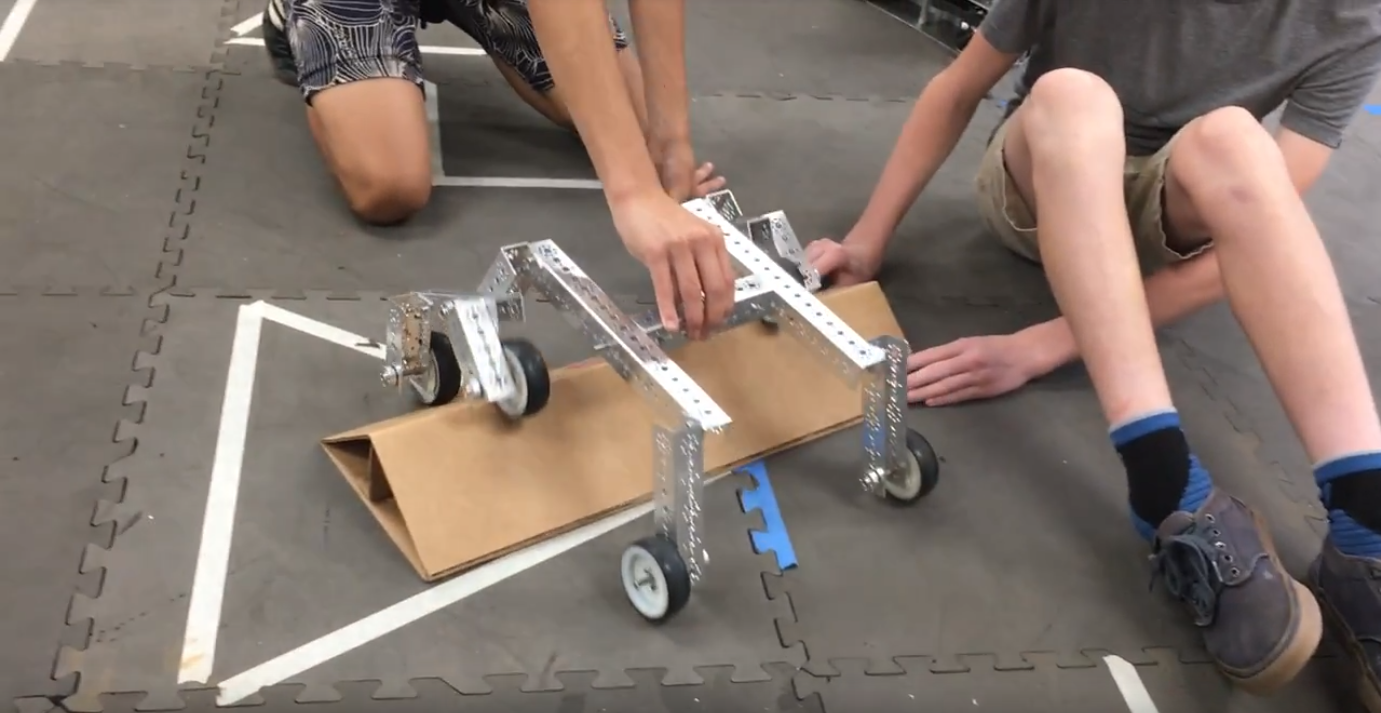
\includegraphics[width=.6\textwidth]{02_09-10/images/Screenshot (5).png}
    \caption{Early Drive train prototype}
    \label{fig:drivetrain sketches}
\end{figure}



\subsection{Develop Drivetrain Prototypes}
%! Work on a drivetrain prototype at the Build Weekend.
Shawn and Ben worked on developing a rocker bogie drivetrain to test. The drivetrain used two different rotation points on both sides to be able to get over things, such as the crater wall. They used a picture from the Internet to assist in the construction of the drivetrain. After it was finished, the drivetrain worked as expected but wasn't quite within the size constraints. Sadly, the drivetrain had to be taken apart. 


\end{document}